%; whizzy paragraph -pdf xpdf -latex ./whizzypdfptex.sh
%; whizzy-paragraph "^\\\\begin{frame}\\|\\\\emtext"
% latex beamer presentation.
% platex, latex-beamer $B$G%3%s%Q%$%k$9$k$3$H$rA[Dj!#(B 

%     Tokyo Debian Meeting resources
%     Copyright (C) 2012 Junichi Uekawa

%     This program is free software; you can redistribute it and/or modify
%     it under the terms of the GNU General Public License as published by
%     the Free Software Foundation; either version 2 of the License, or
%     (at your option) any later version.

%     This program is distributed in the hope that it will be useful,
%     but WITHOUT ANY WARRANTY; without even the implied warreanty of
%     MERCHANTABILITY or FITNESS FOR A PARTICULAR PURPOSE.  See the
%     GNU General Public License for more details.

%     You should have received a copy of the GNU General Public License
%     along with this program; if not, write to the Free Software
%     Foundation, Inc., 51 Franklin St, Fifth Floor, Boston, MA  02110-1301 USA

\documentclass[cjk,dvipdfmx,12pt]{beamer}
\usetheme{Tokyo}
\usepackage{monthlypresentation}

%  preview (shell-command (concat "evince " (replace-regexp-in-string "tex$" "pdf"(buffer-file-name)) "&")) 
%  presentation (shell-command (concat "xpdf -fullscreen " (replace-regexp-in-string "tex$" "pdf"(buffer-file-name)) "&"))
%  presentation (shell-command (concat "evince " (replace-regexp-in-string "tex$" "pdf"(buffer-file-name)) "&"))

%http://www.naney.org/diki/dk/hyperref.html
%$BF|K\8l(BEUC$B7O4D6-$N;~(B
\AtBeginDvi{\special{pdf:tounicode EUC-UCS2}}
%$B%7%U%H(BJIS$B7O4D6-$N;~(B
%\AtBeginDvi{\special{pdf:tounicode 90ms-RKSJ-UCS2}}

\newenvironment{commandlinesmall}%
{\VerbatimEnvironment
  \begin{Sbox}\begin{minipage}{1.0\hsize}\begin{fontsize}{8}{8} \begin{BVerbatim}}%
{\end{BVerbatim}\end{fontsize}\end{minipage}\end{Sbox}
  \setlength{\fboxsep}{8pt}
% start on a new paragraph

\vspace{6pt}% skip before
\fcolorbox{dancerdarkblue}{dancerlightblue}{\TheSbox}

\vspace{6pt}% skip after
}
%end of commandlinesmall

\title{$BEl5~%(%j%"(BDebian$BJY6/2q(B}
\subtitle{$BBh(B109$B2s(B 2014$BG/(B2$B7nEY(B}
\author{$BLnEg5.1Q(B}
\date{2014$BG/(B2$B7n(B14$BF|(B}
\logo{
\includegraphics[width=8cm]{image200607/openlogo-light.eps}}

\begin{document}

\begin{frame}
\titlepage{}
\end{frame}

\begin{frame}{$B@_1D=`Hw$K$46(NO$/$@$5$$!#(B}
$B2q>l@_1D$h$m$7$/$*$M$,$$$7$^$9!#(B
\end{frame}

\begin{frame}{Agenda}
 \begin{minipage}[t]{0.45\hsize}
  \begin{itemize}
   \item $BCm0U;v9`(B
	 \begin{itemize}
	  \item $B<L??$O%;%_%J!<%k!<%`Fb$N$_2D$G$9!#(B
          \item $B=PF~$j$O<+M3$G$J$$$N$G!"$b$730=P$7$?$$J}$O!"LnEg$^$G0l@<$/$@$5$$$^$;!#(B
	 \end{itemize}
   \item $B:G6a$"$C$?(BDebian$B4XO"$N%$%Y%s%HJs9p(B
	 \begin{itemize}
	  \item $BBh(B108$B2s(B $BEl5~%(%j%"(BDebian$BJY6/2q(B
	 \end{itemize}
  \end{itemize}
 \end{minipage} 
 \begin{minipage}[t]{0.45\hsize}
  \begin{itemize}
   \item Debian Trivia Quiz
   \item dnsmasq
  \end{itemize}
 \end{minipage}
\end{frame}

\section{$B%$%Y%s%HJs9p(B}
\emtext{$B%$%Y%s%HJs9p(B}

\begin{frame}{$BBh(B108$B2s(B $BEl5~%(%j%"(BDebian$BJY6/2q(B}

 $BEl5~%(%j%"(BDebian$BJY6/2q(B108$B2sL\$O(B($B3t(B)$B%9%/%&%'%"!&%(%K%C%/%9$5$s$G3+:E$5$l$^$7$?!#(B
5$BL>$N;22C<T$,$"$j$^$7$?!#(B

\begin{itemize}
\item $BLnEg$5$s$,!"(BDebian Pure Blend$B$N>R2p$H!"(BDebian$B$N8x<0%Q%C%1!<%8$K4^$^$l$F$$$k%S%8%e%"%k%N%Y%k%2!<%`MQ$N%Q%C%1!<%8$rNc$KMQ$$!"(BPure Blend$BMQ%Q%C%1!<%8$N:n$jJ}$r>R2p$7$^$7$?!#(B
\item $B;22C<TA40w$G!"3F<+$N:n6H$r9T$$!":G8e$K@.2LH/I=$r$7$^$7$?!#(B
\end{itemize}

 $B:n6H$O$O$+$I$C$?$+$H;W$$$^$9!#$^$?!":G8e$N@.2LH/I=$K$F!"%"%$%G%"6&M-$H$+!"2]Bj$K$D$$$F8l$k$J$I!"$$$m$$$m@9$j>e$,$C$?$H;W$$$^$7$?!#(B

 $B1c2q$O2q>l6a$/$N%?%$5o<r20!V%H%s%?%$!W$K$F9T$$$^$7$?!#(B

\end{frame}

\section{Debian Trivia Quiz}
\emtext{Debian Trivia Quiz}
\begin{frame}{Debian Trivia Quiz}

  Debian $B$N>o<1!"$b$A$m$sCN$C$F$^$9$h$M(B?
$BCN$i$J$$$J$s$FCQ$:$+$7$/$F!"CN$i$J$$$H$O8@$($J$$$"$s$J$3$H$d$3$s$J$3$H!"(B
$B$_$s$J$G3NG'$7$F$_$^$7$g$&!#(B

$B:#2s$N=PBjHO0O$O(B\url{debian-devel-announce@lists.debian.org},
\url{debian-devel@lists.debian.org} $B$KEj9F$5$l$?(B
$BFbMF$J$I$+$i$G$9!#(B

\end{frame}

\subsection{$BLdBj(B}
%; whizzy-master ../debianmeetingresume201311.tex
% $B0J>e$N@_Dj$r$7$F$$$k$?$a!"$3$N%U%!%$%k$G(B M-x whizzytex $B$9$k$H!"(Bwhizzytex$B$,MxMQ$G$-$^$9!#(B
%

\santaku
{$B@hF|!"<!4|(BDebian$B$N%P!<%8%g%s$G$"$k(BJessie$B$K$F!"$H$"$k%"!<%-%F%/%A%c$N%5%]!<%H$,BG$A@Z$i$l$^$7$?!#$=$l$O!"$I$N%"!<%-%F%/%A%c!)(B}
{hurd-i386}
{s390x}
{ia64}
{C}
{$BD9$$4V$*Hh$l!*!d(Bia64$B!#(BAMD$B$N@oN,$KIi$1$?!"@$4V$KIi$1$?!#$H$3$m$G!"(Bhurd-i386$B%"!<%-%F%/%A%c$H(Bsparc$B%"!<%-%F%/%A%c$b!"(BRelease Team$B$K$h$l$P$o$j$H33$C$W$A$J>u67$N$h$&$G$9!#;29M!'(B\url{https://lists.debian.org/debian-devel-announce/2014/01/msg00008.html}}

\santaku
{$B:#7n(B2$B7n$"$?$^$K%j%j!<%9$5$l$?(Bstable$BHG$N(BDebian$B$N%P!<%8%g%s$O$$$/$D$G$7$g$&!)(B}
{7.3}
{7.4}
{7.5}
{B}
{wheezy$B;H$$$N?M$OAaB.%"%C%W%G!<%H$@!*:#2s$b%;%-%e%j%F%#$K4X$9$k(BBugfix$B$,<g$G$9!#(B}

\santaku
{Debian$B$N;q;:(B(Asset$B$N;v$G$9(B)$B$rG$$;$k$3$H$N$G$-$k!V?.Mj$KB-$kAH?%(B(Trusted Organization)$B!W$NDj5A$,@hF|%l%S%e!<$5$l$F$$$^$7$?!#?.Mj$KB-$kAH?%$N>r7o$KEv$F$O$^$i$J$$AH?%$O$I$l(B}
{$B8x<0(BDebian$B3+H/<T$,5o$J$$AH?%(B}
{$BAGAa$$1~Ez(B/$BBP1~$,$G$-$kAH?%(B}
{Debian$B<R2q7{>O$HBPN)$7$J$$AH?%(B}
{A}
{$B:G?7HG$O!"(B\url{https://wiki.debian.org/Teams/DPL/TrustedOrganizationCriteria}
$B$K7G:\$5$l$F$$$^$9!#$A$J$_$K!"?.Mj$KB-$kAH?%$,2?$r$9$k$N$+$NDj5A$K$D$$$F$O!"(BDebian$B%W%m%8%'%/%H7{>O$N(B9.4$B>O$K$"$j$^$9!#:#$^$GL@3N$J4p=`$,$J$+$C$?$N$+!)$H$$$&$N$,$A$g$C$H6C$-!#(B}

\santaku
{1/23$B$K(BPC$B%2!<%`$r%M%C%H$GGd$k%5!<%S%9(B(Steam)$B1?1D$GM-L>$J(BValve$B<R$,!"$$$/$D$+$N(BLinux$BBP1~$N%2!<%`$rL5NA$GDs6!$7$^$9$H7h$a$^$7$?!#$I$s$J?M$,BP>]$G$7$g$&$+!)(B}
{$BA4(BDebian$B%f!<%6(B}
{$BA4(BDebian$B8x<03+H/<T(B}
{$BA4(BIT$B4k6H$N(BDebian$B%5!<%P!<@o;N(B}
{B}
{$B$3$l$b%3%_%e%K%F%#$X$N4k6H$N4sIU$NJ}K!$H$7$FLLGr$$$H;W$$$^$7$?!#(B}


\santaku
{Debian$B$N8xJs%A!<%`$,!"%=!<%7%c%k%a%G%#%"$N8x<0%"%+%&%s%H$G$NH/8@$9$kFbMF$NJg=8$r$7$F$$$^$9!#:G=i$KEj9F$5$l$k$N$O$I$N%"%+%&%s%H$G$7$g$&$+!)(B}
{twitter$B$N(Bdebian}
{google$B!\$N(Bdebian}
{identi.ca$B$N(Bdebian}
{C}
{debian$B$N%=!<%7%c%k%a%G%#%"$N8x<0%"%+%&%s%H$+$i(BDebian$B$N3hF0$r%"%T$j$?$$?M$O1~Jg$7$F$_$k$HNI$$$H$*$b$$$^$9!#(B\url{https://wiki.debian.org/Teams/Publicity/Identica}}





\section{$B;vA02]Bj(B}
\emtext{$B;vA02]Bj(B}
{\footnotesize
\begin{prework}{ 吉野(yy\_{}y\_{}ja\_{}jp) }
\begin{itemize}
\item DDTSS
\item manpages-ja (まだ片付けられてないです...)
\end{itemize}
\end{prework}

\begin{prework}{ dictoss(杉本 典充) }

前回の続きを行う予定です(mpd5をkfreebsdで動くようにデバッグする)

\end{prework}

\begin{prework}{ Yosuke }
cl-quicklispパッケージを理解する。
\end{prework}

}

\section{Debian$B$G(Bdnsmasq$B$r;H$&(B}
\emtext{Debian$B$G(Bdnsmasq$B$r;H$&(B}

\begin{frame}{dnsmsq$B$H$O(B}

 pxe/bootp/dhcp/tftp/dns$B%U%)%o!<%@(B/dns$B%5!<%P!<$r0l<j$K0z$-<u$1$k;v$,$G$-$kJXMx$+$D>.$5$J%=%U%H%&%'%"!#(B

$B!!(B\begin{center}
\Large $B%M%C%H%o!<%/%V!<%H$^$o$j$GMW$j$=$&$J5!G=$r5M$a9~$s$@%9%$%9%"!<%_!<%J%$%U$_$?$$$J$b$N!#(B
  \end{center}

\end{frame}

\begin{frame}{$BM=HwCN<1(B}
 $BESCf(Bbr0$B$H$$$&L>A0$N%V%j%C%8(BI/F$B$,=P$F$-$^$9!#<B:]$N:n$jJ}$O!"(B
 $B2a5n$NEl5~%(%j%"(BDebian$BJY6/2q$N(BKDE$B3+H/4D6-$N;qNA(B
\url{http://tokyodebian.alioth.debian.org/pdf/debianmeetingresume201202.pdf}
$B$K5-:\$7$F$^$9$N$G!"9g$o$;$F$4Mw$/$@$5$$$^$;!#(B
\end{frame}

\begin{frame}{DNS$B%U%)%o!<%@$H$7$F;H$&(B}
\begin{figure}[H]
\begin{center}
 \includegraphics[width=0.7\hsize]{image201402/vm-dns-env.eps}
 \caption{dns$B%U%)%o!<%@$,L5$$>l9g(B}\label{fig:vm-env1}
\end{center}
\end{figure}
\end{frame}

\begin{frame}{DNS$B%U%)%o!<%@$H$7$F;H$&(B}
\begin{figure}[H]
\begin{center}
 \includegraphics[width=0.7\hsize]{image201402/vm-dns-env2.eps}
 \caption{dns$B%U%)%o!<%@$,$"$k>l9g(B}\label{fig:vm-env2}
\end{center}
\end{figure}
\end{frame}

\begin{frame}{DNS$B%U%)%o!<%@$H$7$F;H$&(B}
\begin{center}
\Large
$BMW$O(B
$BJ#?t$N2>A[4D6-$r(BLAN$B$G$D$J$0$h$&$JMQES$r;}$AJb$/$N$KBgJQJXMx(B
\end{center}
\end{frame}

\begin{frame}[containsverbatim]{DNS$B%U%)%o!<%@$N:n$jJ}(B}
\begin{description}
\item[Step 1.] dnsmasq$B$rF3F~$7$^$9!#(B
\begin{commandlinesmall}
note-pc$ sudo aptitude install dnsmasq
\end{commandlinesmall}
%$
\item[Step 2.] br0$B$N$_(Blisten$B$9$k$h$&$K$7!"(Bdns$B%U%)%o!<%@$H$7$F$N$_F0:n$9$k$h$&$K@_Dj$7$^$9!#(B
\begin{commandlinesmall}
note-pc$ sudo vi /etc/dnsmasq.d/forwarder.conf
interface=br0
no-dhcp-interface=br0
bind-interfaces
\end{commandlinesmall}
%$
\end{description}
\end{frame}

\begin{frame}[containsverbatim]{DNS$B%U%)%o!<%@$N:n$jJ}(B}
\begin{description}
\item[Step 3.] dnsmasq$B$r%j%9%?!<%H$7$^$9!#(B
\begin{commandlinesmall}
note-pc$ sudo service dnsmasq restart
\end{commandlinesmall}
%$
\item[Step 4.] $BF0:n$r3N$+$a$^$9(B
\begin{commandlinesmall}
$BFCDj$N%]!<%H$@$1$G(BListen$B$7$F$$$k$3$H$r3N$+$a$k(B
note-pc$ sudo netstat -nlp | fgrep dnsmasq
tcp  0 0 127.0.0.1:53  0.0.0.0:*   LISTEN      16955/dnsmasq   
tcp  0 0 192.168.0.1:53  0.0.0.0:* LISTEN      16955/dnsmasq   
udp  0 0 127.0.0.1:53    0.0.0.0:*             16955/dnsmasq   
udp  0 0 192.168.0.1:53  0.0.0.0:*             16955/dnsmasq   
$B<B:]$K(Bdnsmasq$B$r;XDj$7$FL>A0$r0z$$$F$_$k(B
note-pc$ sudo aptitude install dnsutils
note-pc$ dig @192.168.0.1 www.debian.org a
; <<>> DiG 9.9.3-rpz2+rl.13214.22-P2-Debian-1:9.9.3.dfsg.P2-4 <<>> @192.168.0.1 www.debian.org a
; (1 server found)
;; global options: +cmd
...$BCfN,(B...
;; ANSWER SECTION:
www.debian.org.		300	IN	A	5.153.231.4
www.debian.org.		300	IN	A	128.31.0.51
www.debian.org.		300	IN	A	130.89.148.14
...$BCfN,(B...
\end{commandlinesmall}
%$
\end{description}
\end{frame}

\begin{frame}{$B4J0W(BDNS$B%5!<%P!<$N:n$jJ}(B}

 $B<B$O(Bdnsmasq$B$O%G%U%)%k%H$G(B/etc/hosts$B$rFI$_9~$_!"(BDNS$B%5!<%P!<$H$7$F$b(B
$BF0:n$7$F$$$^$9!#$=$N$?$a!"%[%9%H$N(BA$B%l%3!<%I$@$107$($l$PNI$$$h$&$J(B
$B4J0W(BDNS$B%5!<%P!<$H$7$FMxMQ$9$k>l9g$O!"(B
/etc/hosts$B$r$=$N$^$^MxMQ$9$k$N$,0lHV4JC1$G$9!#(B

\end{frame}

\begin{frame}[containsverbatim]{$B4J0W(BDNS$B%5!<%P!<$N:n$jJ}(B}

\begin{commandlinesmall}
# Host$B%l%3!<%I$NDj5A$NNc"-(B
note-pc$ sudo vi /etc/hosts
-----------/etc/hosts$B$3$3$+$i(B---------------
192.168.0.3 debian0
192.168.0.4 debian1.my-domain debian1
192.168.0.5 debian2.my2-domain debian2
-----------/etc/hosts$B$3$3$^$G(B---------------
# dnsmasq$B:F5/F0$7$F(B/etc/hosts$BFI$^$;$k(B
note-pc$ sudo service dnsmasq restart
# DNS$B$H$7$F0z$$$F$_$k(B
note-pc$ dig @192.168.0.1 debian0 +short
192.168.0.3 ($B"+@5$7$/JV5Q$5$l$F$$$k(B)
note-pc$ dig @192.168.0.1 debian1.my-domain +short
192.168.0.4 ($B"+@5$7$/JV5Q$5$l$F$$$k(B)
note-pc$ dig @192.168.0.1 debian2.my2-domain +short
192.168.0.5 ($B"+>e$H$O0[$J$k%I%a%$%s=jB0$N%l%3!<%I$b@5$7$/JV5Q$5$l$F$$$k(B)
note-pc$ dig @192.168.0.1 debian2 +short
192.168.0.5 ($B"+%[%9%HL>$@$1$G$b@5$7$/JV5Q$5$l$F$$$k(B)
\end{commandlinesmall}

\end{frame}

\begin{frame}[containsverbatim]{$B4J0W(BPXE$B%V!<%H%5!<%P!<$N:n$jJ}(B}
\small
\begin{commandlinesmall}
note-pc$ cd /etc/dnsmasq.d/
note-pc$ sudo rm -f *
note-pc$ sudo vi /etc/dnsmasq.d/pxeboot.conf
----- pxeboot.conf$B$NCf?H(B-----
interface=br0
bind-interfaces
dhcp-range=192.168.0.129,192.168.0.254,255.255.255.0,1h
dhcp-boot=pxelinux.0,pxeserver
pxe-service=x86PC, "Install Linux", pxelinux
enable-tftp
tftp-root=/home/your/srv/tftp
----- pxeboot.conf$B$NCf?H(B-----
note-pc$ cd /home/your/
note-pc$ mkdir srv;mkdir tftp
note-pc$ cd srv/tftp
note-pc$ wget http://ftp.debian.or.jp/debian/dists
   /stable/main/installer-amd64/current/images/netboot/netboot.tar.gz
note-pc$ tar xzf netboot.tar.gz
\end{commandlinesmall}
%$
\end{frame}
\begin{frame}[containsverbatim]{$B4J0W(BPXE$B%V!<%H%5!<%P!<$N:n$jJ}(B}
\small
\begin{commandlinesmall}
note-pc$ sudo service dnsmasq restart
note-pc$ sudo qemu-img create -f raw /var/lib/libvirt/images/debian-pxe 5G
note-pc$ sudo virt-install --connect=qemu:///system -n debian-pxe --ram 512 \
           --pxe --disk /var/lib/libvirt/images/debian-pxe,bus=virtio,size=5,format=raw,cache=writeback \
           --bridge=br0,model=virtio --vnc --hvm --accelerate
\end{commandlinesmall}
%$
\end{frame}

\begin{frame}{$B=*$o$j$K(B}

 $B:#2s$3$3$G$O!"4J0W(Bdns$B%U%)%o!<%@!"4J0W(Bdns$B%5!<%P!<!"4J0W(Bpxe$B%5!<%P!<(B
$B$r(Bdnsmasq$B$r;H$C$FAH$_N)$F$^$7$?!#(B

$B!!$7$+$7!"(Bman dnsmasq$B$rFI$`$HH=$kDL$j!"$b$C$HJ#;($J;v$b4JC1$K=PMh$^$9!#(B
$B$^$?!"<+J,$O$^$C$?$/L$I>2A$G$9$,!":G6a$G$O(Blua$B8@8l$H9g$o$;$F;H$&;v$,$G$-$k$h$&$G$9!#(B

$B!!J#?t$N2>A[4D6-$r;H$C$F%N!<%H(BPC$B>e$KJ#?t$N(BDebian$B$N3+H/4D6-$rN)$A>e$2$k>l9g$K!"(B
$BHs>o$KJXMx$G$9!#(Bdnsmasq$B$r$<$R0lEY$*;n$7$"$l!#(B
>>>>>>> newly add articles tokyo debian meeting

\end{frame}

\section{$B:#8e$N%$%Y%s%H(B}
\emtext{$B:#8e$N%$%Y%s%H(B}
\begin{frame}{$B:#8e$N%$%Y%s%H(B}
\begin{itemize}
 \item 2014$BG/(B3$B7n(B1$BF|(B OSC Tokyo/Spring 2014 $BEl5~%(%j%"(BDebian$BJY6/2q=PD%HG(B
 \item 2014$BG/(B3$B7n(B15$BF|(B $BEl5~%(%j%"(BDebian$BJY6/2q$d$k!)(B
\end{itemize}
\end{frame}

\section{$B:#F|$N1c2q>l=j(B}
\emtext{$B:#F|$N1c2q>l=j(B}
\begin{frame}{$B:#F|$N1c2q>l=j(B}
$BL$Dj(B
\end{frame}

\end{document}

;;; Local Variables: ***
;;; outline-regexp: "\\([ 	]*\\\\\\(documentstyle\\|documentclass\\|emtext\\|section\\|begin{frame}\\)\\*?[ 	]*[[{]\\|[]+\\)" ***
;;; End: ***
